\documentclass[12pt]{article}

\usepackage[ngerman]{babel}
\usepackage[utf8]{inputenc}
\usepackage[T1]{fontenc}
\usepackage[a4paper,lmargin={2cm},rmargin={2cm},tmargin={2.5cm},bmargin={2.5cm}]{geometry}
\usepackage{amssymb}
\usepackage{amsthm}
\usepackage{graphicx}

\usepackage[%
    bookmarks,%
    bookmarksopen=true,%
    pdfauthor={Yannik Bürkle},%
    pdftitle={Proseminar Wirtschaft Schufa},%
    ]{hyperref}

\begin{document}

\begin{titlepage}
\title{Proseminar Wirtschaft\\Schufa}
\author{Yannik Bürkle}
\date{30. Juni 2016}
\end{titlepage}
\maketitle

\newpage

\tableofcontents

\newpage






\section{Einführung}
\begin{figure}[htbp]
    \centering
    
\includegraphics[width=0.8\linewidth]{Schufa_Logo}
    \caption{Schufa Logo}
\end{figure}

Die Schufa Holding AG ist eine privatwirtschaftliche deutsche Wirtschaftsauskunftei. Ihre Hauptaktionäre 
sind vor allem Kreditinstitute, Handelsunternehmen und sonstige Dienstleister.
Das Hauptziel der Schufa ist das Versorgen der Vetragspartner mit Informationen zur Bonität Dritter.\\

Die Schufa besitzt 728 Millionen Einzeldaten über 66,3 Millionen Natürliche Personen und 4,3 Millionen Unternehmen. Jährlich gehen etwa 120 Millionen Anfragen ein, davon 2 Millionen Eigenauskünfte
(siehe Abschnitt \ref{sec:eigenauskunft}). Sie beschäftigt 750 Mitrbeiter und hat einen jährlichen Umsatz von 123 Millionen Euro.


\section{Geschichte}
Die Berliner Städtische Elektrizitätsgesellschaft, kurz Bewag, verkaufte in den 1920er-Jahren nicht nur Strom, sondern auch Haushaltsgeräte in einem Ratenkredit.
Die Rückzahlung der Kredite erfolgte zusammen mit der monatlichen Stromrechnung. Über die Stromrechnung konnte die Bewag schon vor Gewährung des Kredits feststellen, 
ob ein Kunde kreditwürdig ist. Die Kredite wurden entsprechend nur an Kunden herausgegeben, die ihre Rechnungen regelmäßig zahlten.

Dies war das erste System zur Beurteilung des Zahlungsverhaltens Dritter, weshalb zwei leitende Mitarbeiter der Bewag 1927 die \textit{Schutzgemeinschaft für Absatzfinanzierung} gründeten.
In den darauffolgenden Jahren gründeten sich dreizehn weitere regionale Schufa-Gesellschaften, die sich 1952 zur \textit{Bundes-Schufa e.V.} in West-Deutschland zusammenschlossen.

48 Jahre später wurde die Bundes-Schufa e.V. in die heutige Schufa Holding AG umgewandelt und die Anteile der, mittlerweile nur noch acht, Regionalgesellschaften an die Holding übertragen.






\section{Datenspeicherung}
\label{sec:datenspeicherung}
Im Jahr 1970 hat die Schufa ihre komplette Kartei digitalisiert, weshalb diese seit 1977 unter das Bundesdatenschutzgesetz fällt.

Acht Jahre später haben Verbraucherschützer das sogenannte \textit{Schufa-Urteil} erwirkt. Der Bundesgerichtshof entschied, Kundendaten dürfen nur das an die Schufa übermittelt werden, wenn die 
Kunden zuvor entsprechend darüber informiert wurden und sie damit einverstanden sind\footnote{BGH-Urteil vom 19. September 1985}. Aus diesem Urteil entwickelte sich sie sogenannte Schufa-Klausel,
die heutzutage auf nahezu jedem Kredit- und Laufzeitvertrag zu finden ist.

Einige von der Schufa gespeicherten Daten entstammen öffentlichen Bekanntmachungen und Verzeichnissen, die entsprechend nicht unter das Datenschutzgesetz fallen.



\subsection{Gespeicherte Daten}
\label{subsec:gespeicherte-daten}
Die Schufa speichert zur Feststellung der Kreditwürdigkeit folgende Daten:

\subsubsection*{Allgemeine Daten}
Die allgemeinen Daten dienen dazu, eine Person zweifelsfrei zu identifizieren und einer Schufa-Akte zuordnen zu können. Diese Daten können auch ohne Einwilligung an die Vertragspartner herausgegeben 
werden.\\

Die allgemeinen Daten bestehen aus
\begin{itemize}
\item Vor- und Zuname
\item Geburtsdatum und -ort
\item Ggf. Mädchen-/Geburtsname
\end{itemize}

Außerdem speichert die Schufa die aktuelle und auch frühere Anschriften. Wie viele frühere Anschriften und für wie lange ist nicht bekannt.\\

\textit{Diese Daten gehen als neutral in die Schufa-Akte ein.}



\subsubsection*{Art, Gegenstand und Zahlungsbedingungen des jeweiligen Geschäfts}
In diesem Abschnitt gehen alle abgeschlossenen Kredit- und Leasingverträge, alle eröffneten Konten und Kreditkarten und Telekommunikationskonten, also Laufzeitverträge, ein.
Außerdem werden alle Kundenkonten des Handels, also die der Schufa-Vertragspartner, erfasst.\\

\textit{Diese Daten gehen in der Regel als neutral in die Schufa-Akte ein.}



\subsubsection*{Abweichende Zahlungsverhalten}
Unter den abweichenden Zahlungverhalten versteht man Forderungen, die fällig, ausreichend gemahnt und nicht bestritten sind, oder Forderungen nach gerichtlicher Entscheidung.
Anders ausgedrückt sind es schlicht nicht bezahlte Rechnungen oder Lastschriften, welche, zum Beispiel aufgrund mangelnder Kontodeckung, nicht gebucht worden sind.\\

\textit{Diese Daten gehen als negativ in die Schufa-Akte ein.} 



\subsubsection*{Missbrauch von Konten/Kreditkarten nach Nutzungsverbot}
Während eines laufenden Privatinsolvenzverfahrens werden alle Kontobewegungen durch einen Treuhänder überwacht. Die betreffende Person bekommt von ihrem Gehalt nur einen festgelegten Teil zur freien 
Verfügung ausbezahlt, der Rest wird vom Treuhänder an die Schuldner verteilt. Das heißt also für die Person, sie darf ihre Konten und Kreditkarten nicht \glqq missbrauchen\grqq.
Sollte die Person trotzdem Zahlungen über ein gesperrtes Konto tätigen, wird dies auch in der Schufa-Akte vermerkt.\\

\textit{Diese Daten gehen als negativ in die Schufa-Akte ein.}



\subsubsection*{Angaben aus öffentlichen Verzeichnissen und amtlichen Bekanntmachungen}
Dies können zum Beispiel Informationen aus Schuldnerverzeichnissen sein. Weiterhin werden Zwangsvollstreckungsbescheide und Informationen über ein mögliches Privatinsolvenzverfahren und dessen Verlauf erfasst.\\

\textit{Diese Daten gehen als negativ in die Schufa-Akte ein.}\\

Zusätzlich speichert die Schufa, wann welcher Vertragspartner eine Anfrage an die Schufa-Akte gestellt hat. Angaben zum aktuellen Kontostand oder der Höhe des Einskommens werden, im Gegensatz zur Meinung 
vieler Schufa-Kritiker, nicht gespeichert. Die Schufa hat auf diese Daten gar keinen Zugriff.





\subsection{Löschung der Daten}
Im Allgemeinen werden die Schufa-Daten drei Jahre nach ihrer Erledigung, zum Beispiel durch Rückzahlung, gelöscht. Wenn der fällige Betrag 2.000 Euro nicht überschreitet und nach spätestens sechs Wochen 
beglichen wird, wird der entsprechende Eintrag sofort aus der Schufa-Akte entfernt.

Bei Minderjährigen werden beglichene Einträge, unbeachtet deren Dauer, unverzüglich gelöscht.

Daten, die sich auf Bank- und Handelskonten beziehen werden erst mit Auflösung des Kontos entfernt.



Löschung der Daten im Normalfall nach 3 Jahren.






\section{Geschäftspartner}

\subsection{Kategorien der Vertragspartner}

\subsubsection{A-Vertragspartner}
A-Vertragspartner sind Kreditkartenunternehmen, Kreditinstitute und Leasinggesellschaften. Diese erhalten Positiv- und Negativmerkmale aus der Schufa-Akte.

\subsubsection{B-Vertragspartner}
B-Vertragspartner sind Nicht-Banken, also Vetreter aus Handel, Immobilienwirtschaft, Telekommunikationsunternehmen und sonstiger Kreditgebender Unternehmen. Diese erhalten nur die Negativmerkmale.

\subsubsection{F-Vertragspartner}
F-Vertragspartner sind Inkassounternehmen. Diese erhalten ausschließlich Adressdaten. Nach eigenen Angaben gibt die Schufa an Inkassounternehmen nur Adressdaten Natürlicher Personen heraus.



\subsection{Adult Verification System}
Die Schufa bietet neben dem Scoring (siehe Abschnitt \ref{sec:scoring}) noch weitere Dienste an, unter anderem das \textit{Adult Verification System}.
Dieses wird von unter anderem verschiedenen Auktionshäusern und Freemail-Anbietern genutzt. Seit 2005 ist es von der Kommision für Jugendmedienschutz genehmigt und anerkannt.
Wie der Name schon aussagt, handelt es sich hierbei um ein System um das Alter einer (Natürlichen) Person zu überprüfen.

Wer im Internet Produkte mit einer Altersbeschränkung unter 18 verkauft, muss nach dem Jugendschutzgesetz sicherstellen, dass Personen unter 18 diese Produkte nicht kaufen können.
Für Diensteanbieter im Internet ist dies allerdings sehr schwierig, da eine Eingabe ala \glqq Geben Sie hier Ihr Geburtsdatum ein um Ihr Alter zu verifizieren\grqq nicht reicht, sondern
die Altersprüfung \glqq face-to-face\grqq mit einem Ausweis durchgeführt werden muss. Bisher gab es nur \textbf{eine} einfache Möglichkeit namens \textit{PostIdent-Verfahren}. Hierzu muss der Postmitarbeiter 
beim Zustellen des Pakets den Ausweis des Empfängers verlangen, um das Alter zu überprüfen. Dieses Verfahren ist für die Post also recht aufwendlich und daher für den Verkäufer teuer. 

Das Schufa Adult Verification System prüft bereits bei der Registrierung im Versandhandel, ob die Person volljährig ist. Dazu werden die ausweisgeprüften Daten der Schufa-Kartei verwendet.




\section{Eigenauskunft}
\label{sec:eigenauskunft}
§34 Bundesdatenschutzgesetz fordert, jede Person hat das Recht Auskunft über die bei Unternehmen gespeicherten Daten zu erhalten und diese Daten ggf. zu korrigieren.
Bei der Schufa kann man deshalb 1 mal pro Jahr schriftlich eine kostenfreie Datenübersicht bestellen, in der steht, welche Unternehmen zuletzt die Schufa-Akte angefragt haben und warum, welche Einträge momentan 
in der Akte stehen und die aktuellen Branchenscores (siehe Abschnitt \ref{subsec:branchenscore}).

Es kann sein, dass der Vermieter einer neuen Wohnung von der Vertragsunterzeichnung Einblicke in die Schufa-Scores des Mieters bekommen möchte, um zu sehen, ob der Mieter pünktlich zahlt.
Dazu kann man online eine \textit{Bonitätsauskunft} bestellen, in der genau solches aufgelistet ist. Es ist also eine erweitere Datenauskunft für 24,95 Euro.

Ein dritter Weg ist ein Abo auf meineschufa.de abzuschließen. Hier kann man jeden Tag seine aktuellen Scores anschauen oder sogar eine SMS/E-Mail-Benachrichtigung aktivieren, wenn die Schufa-Akte 
verändert wurde.
Die Abopreise variieren je nach Paket zwischen 3,95 und 6,95 Euro pro Monat.






\section{Scoring}
\label{sec:scoring}
Das Scoring ist ein Schätzwert für die Wahrscheinlichkeit, dass eine Person einen Kredit bekommt.
In den Score gehen die in Abschnitt \ref{subsec:gespeicherte-daten} angegebenen Daten und u.a. die Anzahl der Wohnungswechsel und Anzahl der Bankkonten ein.
Das genaue Scoring-Verfahren ist allerdings geheim. Angeblich soll es ein logistisches Regressionsmodell,
bestehend aus Eintrittswahrscheinlichkeiten eines Zufallsereignisses mit zwei möglichen Ausgängen, sein.

Entgegen der Meinung vieler Menschen bestimmt die Schufa mit diesen Scorings nicht, ob jemand einen Kredit bekommt. Die Kreditgeber können, basierend auf diesen Scores, \textbf{selbst}
entscheiden, ob sie den Kredit gewähren oder nicht.

\subsection{Basisscore}
Der Basisscore besteht aus einem Wert zwischen 1 und 100 Prozent, wobei höhere Werte besser sind. Die 100\% sind nur in der Theorie erreichbar.\\
Eine Stichprobe unter 100 Personen ergab folgende Durchschnittswerte:

\begin{table}[h!]
	\begin{center}
	\begin{tabular}[c]{lr} \hline
		\textbf{Personengruppe} & \textbf{Score}\\
		\hline
		In Insolvenzverfahren & 5\%\\
		Abgeschlossenes Verfahren & Score 29\%\\
		4 Personen & \textit{kein Score}\\
		9 Personen & <89\%\\
		60 Personen & 89-99\%\\
		27 Personen & >99\%\\
		\hline
	\end{tabular}
	\caption{Durchnittliche Scores bei 100 Personen}
	\end{center}
\end{table}

Der Basisscore wird jedes Quartal neu berechnet.



\subsection{Branchenscore}
\label{subsec:branchenscore}
Der Branchenscore wurde 1997 eingeführt, um, wie der Name bereits aussagt, für jede Branche einen spezifischen Scorewert ermitteln zu können. Der Branchenscore wird tagesaktuell berechnet.
Es gibt zwei Versionen. Version 1.0 von 2001 und Version 2.0 von 2008. Einige Branchen werden in V1.0 berechnet, andere widerum in V2.0.

V1.0 besteht aus Werten von 0 bis 1.000 Punkten, V2.0 ist weiter aufgeschlüsselt und bietet Werte von 0 bis 9.999. Bei beiden Versionen sind höhere Werte besser.\\

Zusätzlich zu den Scorewerten gibt es auch noch die Rankingstufe von A-P, wobei A die beste ist, eine Erfüllungswahrscheinlichkeit, welche ähnlich dem Basisscore in Prozent angegeben ist 
und eine Risikobewertung (siehe Abb. \ref{fig:bsp-branchenscore}).

\begin{figure}[h!]
	\centering
		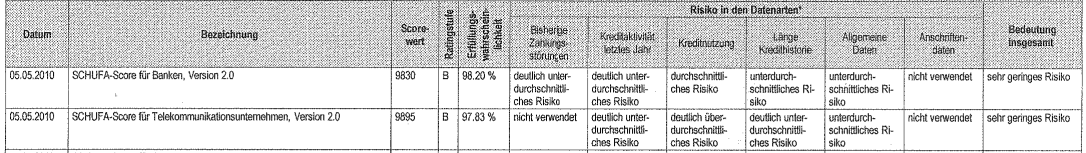
\includegraphics[width=\linewidth]{branchenscore}
	\caption{Beispiel für einen Branchenscore}
	\label{fig:bsp-branchenscore}
\end{figure}






\section{Kritik}

Die Schufa muss seit ihrer Gründung viel Kritik vertragen. Nur zu häufig hört man den Begriff \textit{\textbf{Sch}ulden\textbf{fa}lle} für die Abkürzung Schufa. Im folgenden sind einige Kritikpunkte aufgelistet.
Hauptsächlich kommt die Kritik von Vebraucher- und Datenschützern und Rechtsanwälten. Die Medien greifen dieses Thema auch immer mal wieder auf.

\subsection{Position der Schufa}

Die Schufa hat eine gehobene Stellung unter den Auskunfteien aufgrund der tiefen Beziehung zu Kreditinstituten und der enormen Datenmenge, die sie besitzt. Außerdem ist es nur schwer möglich,
ein Bankkonto oder einen Kredit ohne Unterzeichnung der Schufa-Klausel (siehe Abschnitt \ref{sec:datenspeicherung}) zu bekommen.\\

Die Schufa begründet ihre Stellung dadurch, dass die Bonitätsprüfung nicht nur dem Kreditgeber diene, sondern indirekt durch geringere Risikoprämien auch den Kreditnehmern.

Außerdem schütze die Schufa die Verbraucher vor einer Überschuldung, da gefährdeten Personen erst gar kein weiterer Kredit genehmigt wird. Wie bereits erwähnt hat hier aber der Kreditgeber die 
Entscheidungsgewalt, nicht die Schufa - sie berät nur.\\

Laut einem Bericht des NDR aus dem Jahr 2014 zweifeln die Aufsichtsbehörden mancher Bundesländer an der rechtlichen Zulässigkeit der Schufa. Es gibt hierfür immerhin keine rechtliche Grundlage, auf die sich
die Privatdankenbank stützen kann.

\subsection{Scoring}

Viele beklagen sich darüber, dass die Schufa ihre Scoringmethoden nicht offenlegt. Niemand weiß über die genauen Verfahren bescheid.
Der Bundesgerichtshof erklärt die Geheimhaltung des Schufa-Scoring allerdings für in Ordnung.\\

Bis 2001 war das Einholen einer Eigenauskunft nach dem BDSG als Negativeintrag in der Schufa-Akte hinterlegt, was allerdings nach massiven Protesten eingestellt wurde.\\

Laut einem weiteren NDR-Bericht von 2014 ist in der Schufa-Bewertung wohl das Umzugsverhalten und die Bankkontonutzung sehr wichtig. Wenn eine Person häufig umzieht und/oder viele Bankkonten besitzt,
wirke sich das negativ auf die Kreditwürdigkeit aus. Laut NDR werde dies sogar stärker bewertet als richtige Negativeintragungen wie eine Privatinsolvenz, die erst an fünfter Stelle kommen soll.


\subsection{Fehlerhafte Daten}
Die \textit{Stiftung Warentest} hat 2010 in einer Stichprobe herausgefunden, dass etwa 1\% der Schufa-Daten schlicht falsch, 8\% veraltet und 28\% komplett fehlen.
Die Schufa wehrte die Vorwürfe ab, da sie selbst für die Richtig- und Vollständigkeit der Datensätze nichts kann. Die Vertragspartner seien nach dem Gegenseitigkeitsprinzip dazu verpflichtet,
Aktualisierungen an die Schufa zu melden.

\subsection{Internetrecherchen}
2012 startete die Schufa zusammen mit dem Hasso-Plattner-Institut einen Versuch, ähnlich wie auch heute noch Personaler bei Bewerbungsgesprächen, im Internet nach Informationen über die betreffende
Person zu suchen. Als diese Zusammenarbeit öffentlcih wurde regte sich massiver Widerstand in der Bevölkerung, woraufhin der Vertrag seitens des Instituts gekündigt wurde.

\newpage

\section{Quellenangaben}
\begin{itemize}
\item http://de.wikipedia.org/wiki/Schufa
\item http://www.t-online.de/wirtschaft/id\_67634822/schufa-siegt-vor-dem-bundesgerichtshof-scoring-formel-bleibt-geheim.html
\item https://www.test.de/Auskunfteien-Fehlerhafte-Daten-gespeichert-4047751-0/
\item https://books.google.de/books?id=m1kpBAAAQBAJ\&lpg=PA33\&ots=iIp83FquRf\&dq=bewag\%20haushaltsger\%C3\%A4te\&hl=de\&pg=PA33\#v=onepage\&q=bewag\%20haushaltsger\%C3\%A4te\&f=false
\item https://www.schufa.de/de/unternehmenskunden/leistungen/fraudprevention-compliance/schufa-identitaetscheck-jugendschutz/
\item http://www.ndr.de/der\_ndr/presse/mitteilungen/Neue-bundesweite-Betrugsdatei-der-SchufaDatenschuetzer-zweifeln-an-Zulaessigkeit-,pressemeldungndr14700.html
\item http://www.t-online.de/wirtschaft/id\_68926952/ndr-deckt-geheime-schufa-liste-auf-so-entsteht-der-schufa-score.html
\end{itemize}

\begin{small}
\textit{Dieses Dokument liegt Ihnen in der Version 1.0.0 vom 07.07.2016 vor. Weitere Versionen finden Sie unter \href{url}{https://github.com/yannik-b/proseminar-schufa/releases}.}
\end{small}

\end{document}
